El objetivo de esta guía de usuario es proporcionar a los usuarios un ejemplo para la puesta a punto y ejecución de las 
funcionalidades implementadas en el paquete NPM ghshell durante el Trabajo de Fin de Máster.

%---------------------------------------------------------------------------------
\section{Instalación}
\label{Apendice2:instalacion}

%---------------------------------------------------------------------------------
\subsection{Requisitos}
\label{subsec:b.1.1}

\begin{itemize}
	\item Node.js versión \textgreater = 8:
	
	Descargable desde la página oficial de Node.js (\url{https://nodejs.org/en/download/current/}).
	
\end{itemize}

%---------------------------------------------------------------------------------
\subsection{Dependencias}
\label{subsec:b.1.2}

Para poder generar los libros usando Gitbook, son necesarias las siguientes dependencias:

\begin{itemize}
	\item Paquete de Gitbook (\url{https://www.npmjs.com/package/gitbook-cli}):
	
	Para instalarlo, basta con ejecutar el siguiente comando:
	
	\begin{verbatim}
		[~]$ npm install -g gitbook-cli
	\end{verbatim}

	\item Aplicación Calibre (\url{https://calibre-ebook.com/download})
	
	Para instalarla, basta con ejecutar el siguiente comando:
	
	\begin{verbatim}
		[~]$ sudo aptitude install calibre
	\end{verbatim}
	
	NOTA: en algunas distribuciones GNU/Linux, node es instalado como nodejs, por lo que es necesario crear un enlace simbólico:
	
	\begin{verbatim}
		[~]$ sudo ln -s /usr/bin/nodejs /usr/bin/node
	\end{verbatim}
	
\end{itemize}

%---------------------------------------------------------------------------------
\subsection{Instalación}
\label{subsec:b.1.3}

Para instalar el paquete ghshell, basta con ejecutar el siguiente comando:

\begin{verbatim}
[~]$ npm install -g ghshell
\end{verbatim}

%---------------------------------------------------------------------------------


\section{Ejecución}
\label{Apendice2:ejecucion}

%---------------------------------------------------------------------------------
\subsection{Primeros pasos}
\label{subsec:b.2.1}

Para ejecutar el programa, basta con ejecutar el siguiente comando en la consola:

\begin{verbatim}
[~]$ ghshell
\end{verbatim}

%---------------------------------------------------------------------------------

\subsection{Iniciar/Cerrar sesión}
\label{subsec:b.2.1}
    
    Iniciar o cerrar sesión. Comandos 'login' y 'logout'. 
    
    	\begin{verbatim}
			ghshell > login
			ghshell > logout
		\end{verbatim}
    
    La primera vez que se ejecuta el programa, pedirá directamente el usuario y contraseña de GitHub:
    
    	\begin{figure}[H]
		\begin{center}
		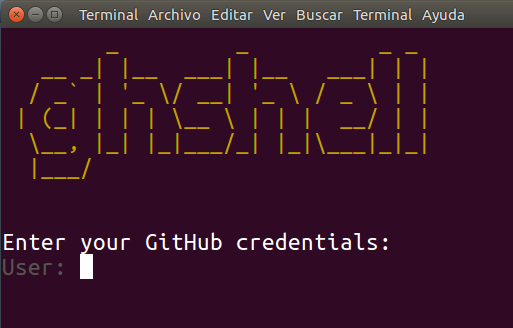
\includegraphics[width=0.7\textwidth]{images/ghshell1}
		\caption{Login de usuario}
		\label{fig:ghshell1}
		\end{center}
		\end{figure}
		
 
 		\begin{figure}[H]
		\begin{center}
		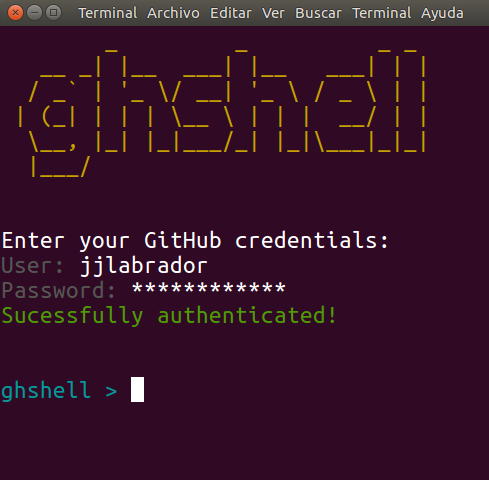
\includegraphics[width=0.6\textwidth]{images/ghshell2-1}
		\caption{Usuario autenticado}
		\label{fig:ghshell2-1}
		\end{center}
		\end{figure}
		
    Una vez que el usuario se autentifica con GitHub, se genera un token personal, que se usa posteriormente para acceder a la API de Github. Este token se almacena cifrado en el equipo del usuario, por lo que las siguientes ocasiones que utilice la herramienta no hará falta que vuelva a iniciar sesión:
        
        \begin{figure}[H]
		\begin{center}
		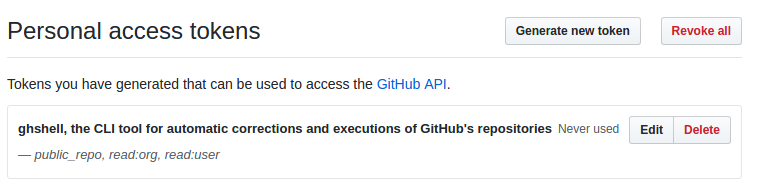
\includegraphics[width=1\textwidth]{images/ghshell2-3}
		\caption{Token personal en GitHub}
		\label{fig:ghshell2-3}
		\end{center}
		\end{figure}
		
		\begin{figure}[H]
		\begin{center}
		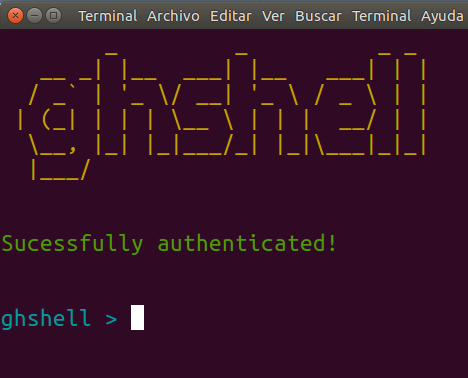
\includegraphics[width=0.6\textwidth]{images/ghshell2-4}
		\caption{Login automático una vez generado el token}
		\label{fig:ghshell2-4}
		\end{center}
		\end{figure}
		
	Si el usuario cierra sesión en la herramienta, se eliminará el token en GitHub y en el equipo:
	
		\begin{figure}[H]
		\begin{center}
		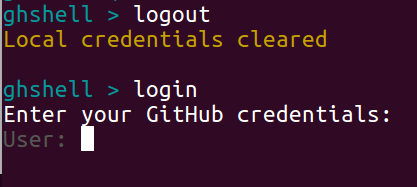
\includegraphics[width=0.6\textwidth]{images/ghshell2-2}
		\caption{Logout de usuario}
		\label{fig:ghshell2-2}
		\end{center}
		\end{figure}
		

%---------------------------------------------------------------------------------

\subsection{Contexto principal}
\label{subsec:b.2.2}

	Una vez autentificados, en el menú principal podremos hacer las siguientes acciones:
	
	\begin{itemize}
		\item Mostrar la ayuda. Comando 'help'.
		
		\begin{verbatim}
			ghshell > help
		\end{verbatim}
		
		En función del contexto donde nos encontremos, se mostrarán diferentes opciones en la ayuda.
		
		\begin{figure}[H]
		\begin{center}
		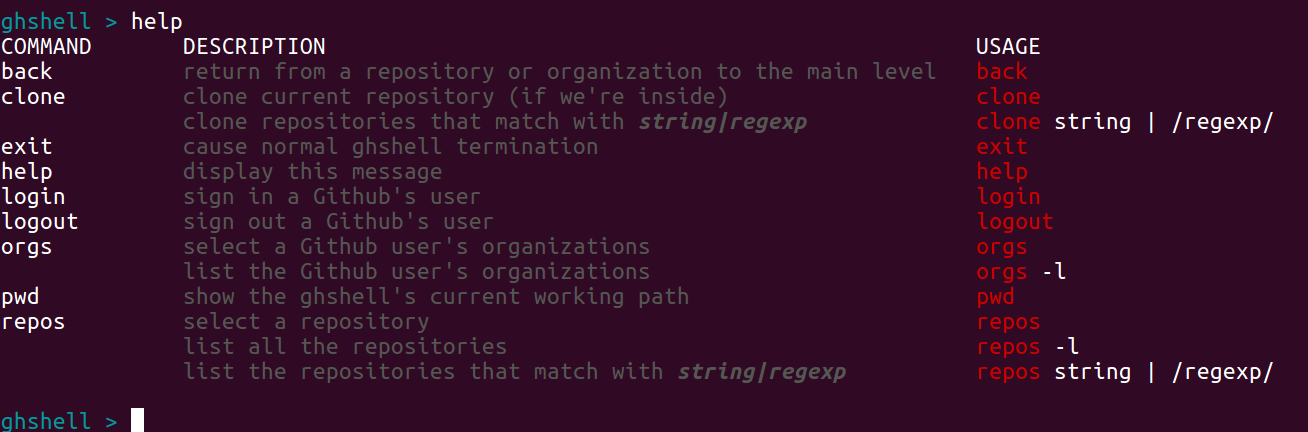
\includegraphics[width=1\textwidth]{images/help1-1}
		\caption{Ayuda global}
		\label{fig:help1-1}
		\end{center}
		\end{figure}
		
		%-------------------
		\item Mostrar el directorio de trabajo actual. Comando 'pwd'.
		
		\begin{verbatim}
			ghshell > pwd
		\end{verbatim}
		
		Visualiza el directorio de trabajo donde se ha ejecutado el programa:
		
		\begin{figure}[H]
		\begin{center}
		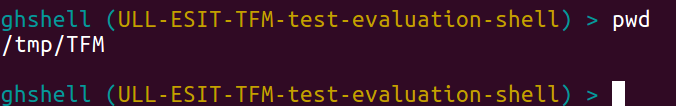
\includegraphics[width=0.7\textwidth]{images/pwd}
		\caption{Directorio actual de trabajo}
		\label{fig:pwd}
		\end{center}
		\end{figure}
		
		NOTA: este comando tiene el mismo comportamiento si nos encontramos dentro de una organización o dentro de un repositorio de una organización.
		
		%-------------------
		\item  Listar y acceder a organizaciones. Comando 'orgs'.
		
		\begin{verbatim}
			ghshell > orgs [-l]
		\end{verbatim}
		
		Si se ejecuta el comando sin argumentos, pregunta al usuario a qué organización quiere acceder. Se puede usar la tecla tabulador para ver las organizaciones disponibles.
		
		\begin{figure}[H]
		\begin{center}
		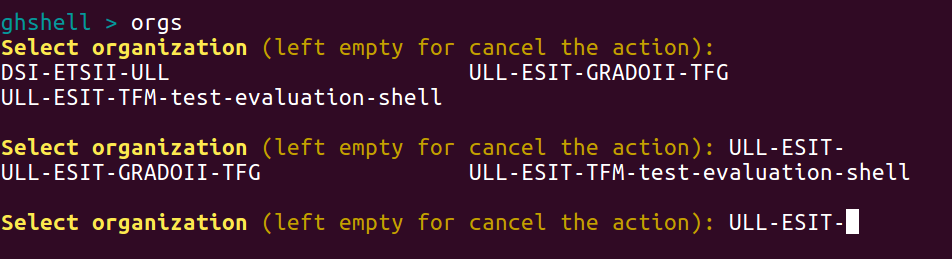
\includegraphics[width=0.8\textwidth]{images/orgs1-1}
		\caption{Acceso a una organización}
		\label{fig:orgs1-1}
		\end{center}
		\end{figure}
		
		El prompt de la consola cambiará para indicarnos que nos encontramos dentro de la organización.
		\bigskip
		
		Si se ejecuta el comando con la opción '-l', simplemente lista las organizaciones a las que pertenece el usuario.
		
		\begin{figure}[H]
		\begin{center}
		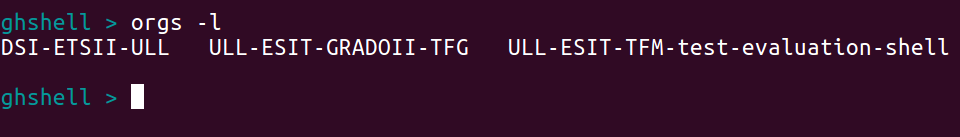
\includegraphics[width=0.8\textwidth]{images/ghshell3}
		\caption{Lista de organizaciones del usuario}
		\label{fig:ghshell3}
		\end{center}
		\end{figure}
				
		%-------------------
		\item  Listar y acceder a repositorios. Comando 'repos'.
		
		\begin{verbatim}
			ghshell > repos [-l] [string | /regexp/]
		\end{verbatim}
		
		Si se ejecuta el comando sin argumentos, pregunta al usuario a qué repositorio quiere acceder. Se puede usar la tecla tabulador para ver los repositorios disponibles.
		
		\begin{figure}[H]
		\begin{center}
		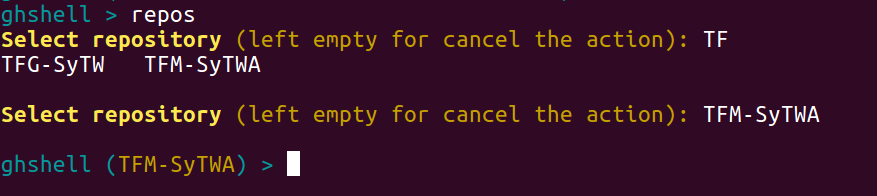
\includegraphics[width=0.8\textwidth]{images/repos1-1}
		\caption{Acceso a un repositorio}
		\label{fig:repos1-1}
		\end{center}
		\end{figure}
		
		
		El prompt de la consola cambiará para indicarnos que nos encontramos dentro de un repositorio.		
		\bigskip
		
		Si se ejecuta el comando con la opción '-l', simplemente se listan los repositorios que pertenecen al usuario.
		
		\begin{figure}[H]
		\begin{center}
		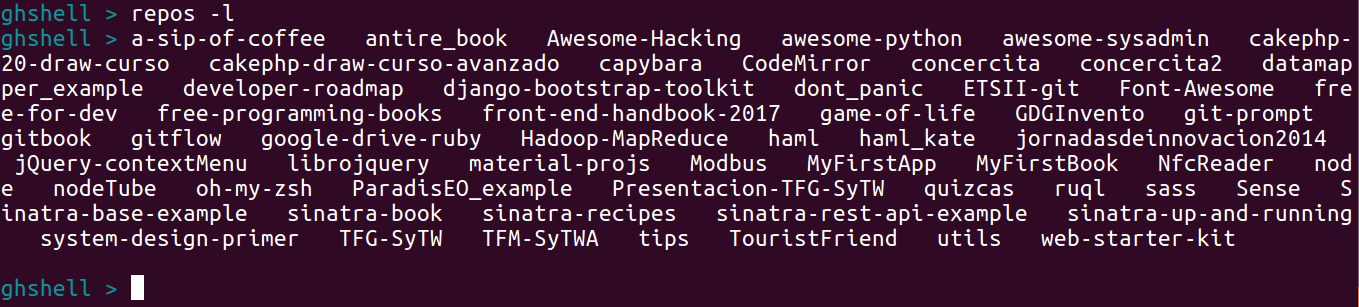
\includegraphics[width=1\textwidth]{images/repos1-2}
		\caption{Listado de repositorios del usuario}
		\label{fig:repos1-2}
		\end{center}
		\end{figure}
		
		Si se especifica como argumento un string o expresión regular, se mostrarán los repositorios que coincidan con ese argumento:
		
		\begin{figure}[H]
		\begin{center}
		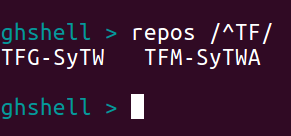
\includegraphics[width=0.4\textwidth]{images/repos1-3}
		\caption{Listado de repositorios del usuario que coinciden con el argumento pasado}
		\label{fig:repos1-3}
		\end{center}
		\end{figure}
		
		
		NOTA: este comando tiene el mismo comportamiento si nos encontramos dentro de una organización.
		
		
		\begin{figure}[H]
		\begin{center}
		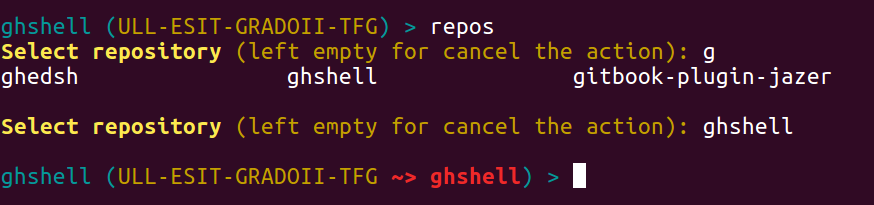
\includegraphics[width=0.9\textwidth]{images/repos1-4}
		\caption{Acceso a un repositorio dentro de una organización}
		\label{fig:repos1-4}
		\end{center}
		\end{figure}
		
		\begin{figure}[H]
		\begin{center}
		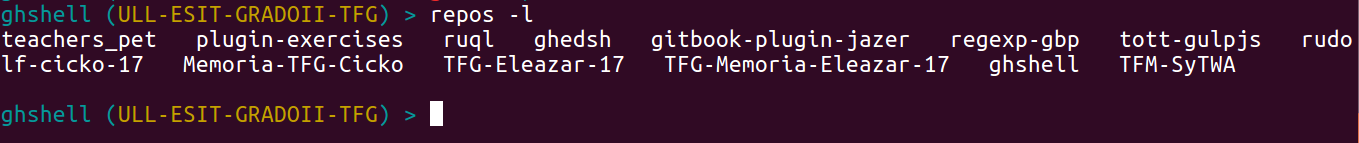
\includegraphics[width=1\textwidth]{images/repos1-5}
		\caption{Listado de repositorios de una organización}
		\label{fig:repos1-5}
		\end{center}
		\end{figure}
		
		\begin{figure}[H]
		\begin{center}
		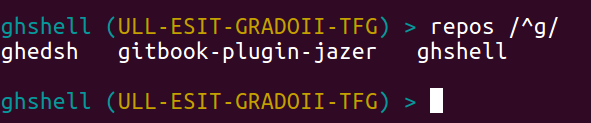
\includegraphics[width=0.7\textwidth]{images/repos1-6}
		\caption{Listado de repositorios de una organización que coinciden con el argumento pasado}
		\label{fig:repos1-6}
		\end{center}
		\end{figure}	
		
		%-------------------
		\item  Clonar repositorios. Comando 'clone'.
		
		\begin{verbatim}
			ghshell > clone string | /regexp/
		\end{verbatim}	
		
		Al especificar el argumento como un string o expresión regular, se clonarán todos los repositorios que coincidan con ese argumento. 
		
		\begin{figure}[H]
		\begin{center}
		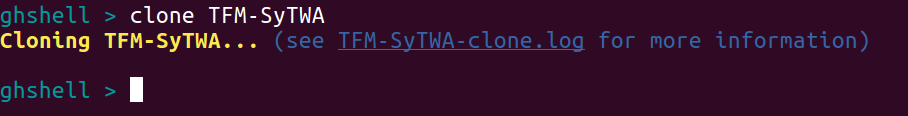
\includegraphics[width=0.9\textwidth]{images/clone1-1}
		\caption{Clonado de repositorios que coinciden con el string pasado}
		\label{fig:clone1-1}
		\end{center}
		\end{figure}
		
		\begin{figure}[H]
		\begin{center}
		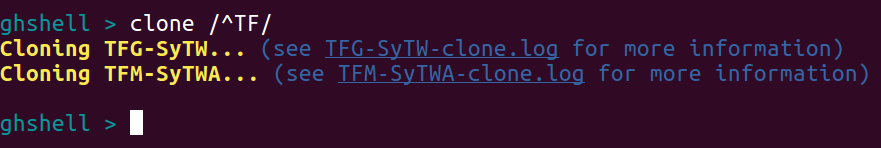
\includegraphics[width=0.9\textwidth]{images/clone1-2}
		\caption{Clonado de repositorios que coinciden con la regexp pasada}
		\label{fig:clone1-2}
		\end{center}
		\end{figure}
		
		
		El clonado se realiza de manera asíncrona, por lo que podemos seguir trabajando mientras se clona(n) el/los repositorio(s). Se puede observar el estado de la clonación revisando el fichero de log que se genera: \textless nombre-repositorio\textgreater -clone.log.:
		
		\begin{figure}[H]
		\begin{center}
		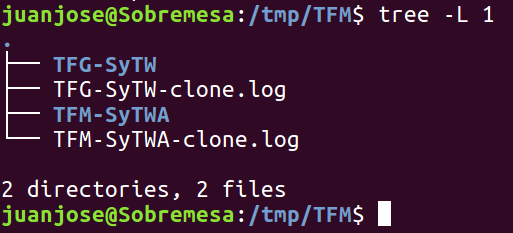
\includegraphics[width=0.7\textwidth]{images/clone1-3}
		\caption{Resultado del clonado de repositorios}
		\label{fig:clone1-3}
		\end{center}
		\end{figure}
		
		
		Los fichero de log muestran la información del clonado. Se ha añadido una huella de tiempo para tener un control más exacto sobre cuándo ocurre cada evento:
		
		\begin{verbatim}
[2017/07/02-01:20:47] Clonar en «TFM-SyTWA»...

[2017/07/02-01:20:48] remote: Counting objects: 92, done.        

[2017/07/02-01:20:48] remote: Compressing objects:   1% (1/65)           
remote: Compressing objects:   3% (2/65)           
remote: Compressing objects:   4% (3/65)           
remote: Compressing objects:   6% (4/65)           
remote: Compressing objects:   7% (5/65)           
remote: Compressing objects:   9% (6/65)           
remote: Compressing objects:  10% (7/65)           
remote: Compressing objects:  12% (8/65)           
remote: Compressing objects:  13% (9/65)           
remote: Compressing objects:  15% (10/65)           
remote: Compressing objects:  16% (11/65)           
remote: Compressing objects:  18% (12/65)           
[2017/07/02-01:20:48] remote: Compressing objects:  20% (13/65)           
remote: Compressing objects:  21% (14/65)           
remote: Compressing objects:  23% (15/65)           
remote: Compressing objects:  24% (16/65)           
remote: Compressing objects:  26% (17/65)           
remote: Compressing objects:  27% (18/65)           
remote: Compressing objects:  29% (19/65)           
remote: Compressing objects:  30% (20/65)           
remote: Compressing objects:  32% (21/65)           
remote: Compressing objects:  33% (22/65)           
remote: Compressing objects:  35% (23/65)           
remote: Compressing objects:  36% (24/65)           
remote: Compressing objects:  38% (25/65)           
remote: Compressing objects:  40% (26/65)           
remote: Compressing objects:  41% (27/65)           
remote: Compressing objects:  43% (28/65)           
remote: Compressing objects:  44% (29/65)           
remote: Compressing objects:  46% (30/65)           
remote: Compressing objects:  47% (31/65)           
remote: Compressing objects:  49% (32/65)           
remote: Compressing objects:  50% (33/65)           
remote: Compressing objects:  52% (34/65)           
remote: Compressing objects:  53% (35/65)           
remote: Compressing objects:  55% (36/65)           
remote: Compressing objects:  56% (37/65)           
remote: Compressing objects:  58% (38/65)           
remote: Compressing objects:  60% (39/65)           
remote: Compressing objects:  61% (40/65)           
remote: Compressing objects:  63% (41/65)           
remote: Compressing objects:  64% (42/65)           
remote: Compressing objects:  66% (43/65)           
remote: Compressing objects:  67% (44/65)           
remote: Compressing objects:  69% (45/65)           
remote: Compressing objects:  70% (46/65)           
remote: Compressing objects:  72% (47/65)           
remote: Compressing objects:  73% (48/65)           
remote: Compressing objects:  75% (49/65)           
remote: Compressing objects:  76% (50/65)           
remote: Compressing objects:  78% (51/65)           
remote: Compressing objects:  80% (52/65)           
remote: Compressing objects:  81% (53/65)           
remote: Compressing objects:  83% (54/65)           
remote: Compressing objects:  84% (55/65)           
remote: Compressing objects:  86% (56/65)           
remote: Compressing objects:  87% (57/65)           
remote: Compressing objects:  89% (58/65)           
remote: Compressing objects:  90% (59/65)           
remote: Compressing objects:  92% (60/65)           
remote: Compressing objects:  93% (61/65)           
remote: Compressing objects:  95% (62/65)           
remote: Compressing objects:  96% (63/65)           
remote: Compressing objects:  98% (64/65)           
remote: Compressing objects: 100% (65/65)           
remote: Compressing objects: 100% (65/65), done.        

[2017/07/02-01:20:49] remote: Total 92 (delta 25), reused 92 (delta 25), pack-reused 0        

[2017/07/02-01:20:49] Comprobando la conectividad… 
[2017/07/02-01:20:49] hecho.

\end{verbatim}
		
		%-------------------		
		\item  Salir del programa. Comando 'exit'.
		
		Causa el cierre ordenado del programa.
		
		NOTA: este comando tiene el mismo comportamiento si nos encontramos dentro de una organización o dentro de un repositorio de una organización. 
		
	\end{itemize}

\subsection{Contexto de organización}
\label{subsec:b.2.2}

	Los comandos 'pwd', 'repos', 'clone' y 'exit' tienen el mismo comportamiento que en el contexto principal. 
	\bigskip
	Además, en el caso del comando 'clone', se creará una carpeta con el nombre de la organización en la que nos encontremos y en ella se guardarán todos los repositorios clonados.
	
	%-------------------
\begin{itemize}

	\item Mostrar la ayuda. Comando 'help'.
		
		\begin{verbatim}
			ghshell > help
		\end{verbatim}
		
		En función del contexto donde nos encontremos, se mostrarán diferentes opciones en la ayuda.
		
		\begin{figure}[H]
		\begin{center}
		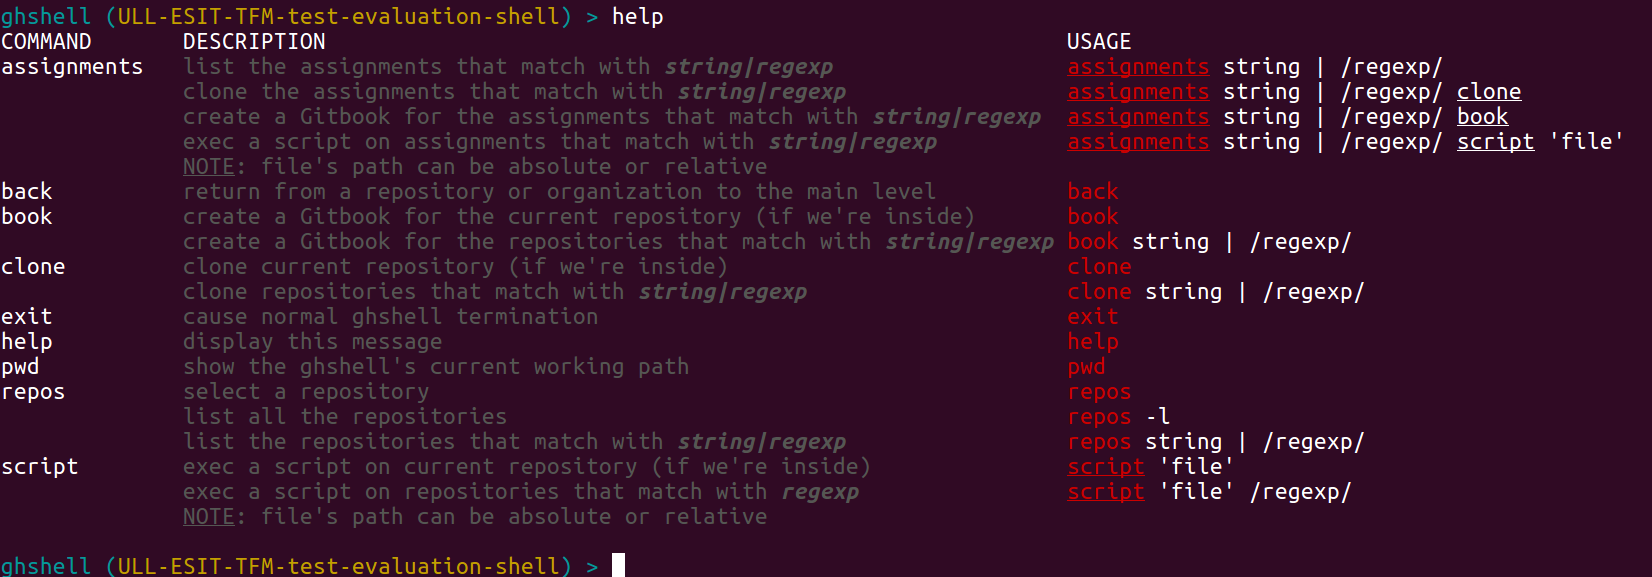
\includegraphics[width=1\textwidth]{images/help1-2}
		\caption{Ayuda en el contexto de organización}
		\label{fig:help1-2}
		\end{center}
		\end{figure}
	
	%-------------------	
	\item Salir del contexto actual. Comando 'back'.
	
		\begin{verbatim}
			ghshell > back
		\end{verbatim}
		
		Si nos encontramos en un repositorio propio o en una organización, regresamos al contexto principal. Si nos encontramos dentro de un repositorio de una organización, regresamos al contexto de la organización.
		
		\begin{figure}[H]
		\begin{center}
		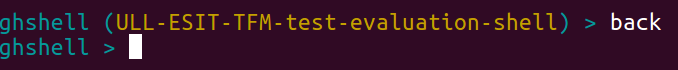
\includegraphics[width=0.7\textwidth]{images/back1-1}
		\caption{Regreso al contexto principal desde una organización}
		\label{fig:back1-1}
		\end{center}
		\end{figure}
		
		\begin{figure}[H]
		\begin{center}
		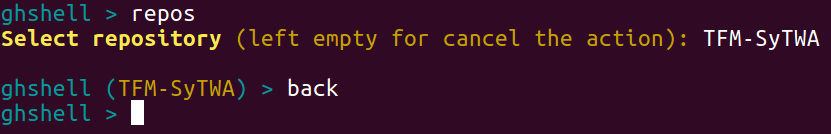
\includegraphics[width=0.8\textwidth]{images/back1-2}
		\caption{Regreso al contexto principal desde un repositorio}
		\label{fig:back1-2}
		\end{center}
		\end{figure}
		
	%-------------------	
	\item Ejecutar un script determinado. Comando 'script'.
	
		\begin{verbatim}
			ghshell > script <file> /regexp/
		\end{verbatim}
		
	Este comando sirve para ejecutar un script. La ruta del fichero del script puede ser absoluta o relativa.
	
	Al especificar una expresión regular, se ejecutará el script en todos los repositorios que coincidan con la expresión regular indicada.
	
		\begin{figure}[H]
		\begin{center}
		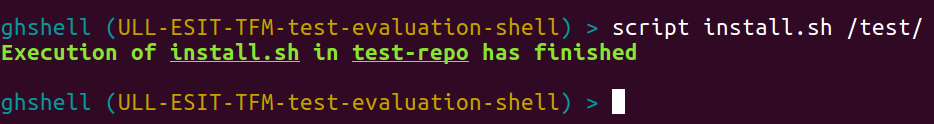
\includegraphics[width=0.8\textwidth]{images/script1-1}
		\caption{Ejecución de script en repositorios que coinciden con la regexp pasada}
		\label{fig:script1-1}
		\end{center}
		\end{figure}
		
	
	La ejecución de cada script se ejecuta en un proceso hijo independiente pero, a diferencia del clonado, el script se ejecuta línea a línea de manera síncrona. Se puede observar el estado de la ejecución del script y los resultados revisando el fichero de log que se genera: \textless nombre-repositorio \textgreater - \textless nombre-script \textgreater .log
	
		\begin{figure}[H]
		\begin{center}
		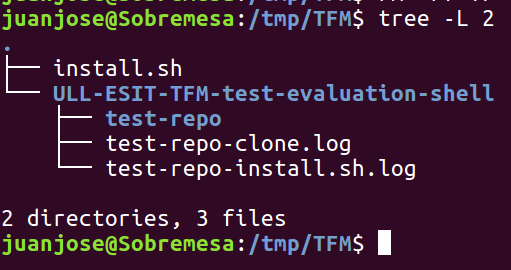
\includegraphics[width=0.7\textwidth]{images/script1-2}
		\caption{Fichero de log generado resultante de la ejecución del script}
		\label{fig:script1-2}
		\end{center}
		\end{figure}
	
	%-------------------
	\item Exportar resultados. Comando 'book'.
	
		\begin{verbatim}
			ghshell > book string | /regexp/
		\end{verbatim}
	
	Este comando genera un Gitbook con los resultados de todos los scripts ejecutados sobre los repositorios. Este libro se genera en formato PDF y en HTML.
	
	Al especificar un string o expresión regular, se creará el libro por cada repositorios que coincida con la expresión regular indicada.
	
		\begin{figure}[H]
		\begin{center}
		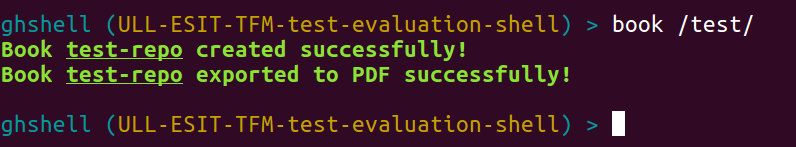
\includegraphics[width=0.8\textwidth]{images/book1-1}
		\caption{Creación del Gitbook en repositorios que coinciden con la regexp pasada}
		\label{fig:book1-1}
		\end{center}
		\end{figure}
		
	
	La creación del libro se realiza de manera asíncrona, por lo que se puede seguir trabajando mientras se genera. Se puede observar el estado de la creación del libro y su exportación a PDF revisando los ficheros de logs que se generan:
	\textless nombre-repositorio \textgreater -gitbook{\_}build.out y \textless nombre-repositorio \textgreater -gitbook{\_}pdf.out.
	\bigskip
	
    La carpeta que contiene el libro en HTML se llamará \textless nombre-repositorio\textgreater {\_}gitbook. El fichero PDF se llamará \textless nombre-repositorio\textgreater .pdf.
	
		\begin{figure}[H]
		\begin{center}
		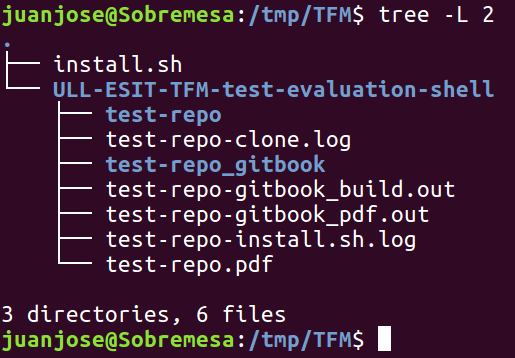
\includegraphics[width=0.7\textwidth]{images/book1-2}
		\caption{Directorios y ficheros generados del Gitbook}
		\label{fig:book1-2}
		\end{center}
		\end{figure}
	
	%-------------------	 
	\item Seleccionar assignments. Comando 'assignments'.
	
		\begin{verbatim}
			ghshell > assignments string | /regexp/ [clone|book|script <file>]
		\end{verbatim}
		
		Los assignments son tratados como un caso especial de repositorios dentro de una organización.
		
		Si sólo se pasa como argumento un string o una expresión regular, listará los assignments que coincidan con dicho argumento.
		
		\begin{figure}[H]
		\begin{center}
		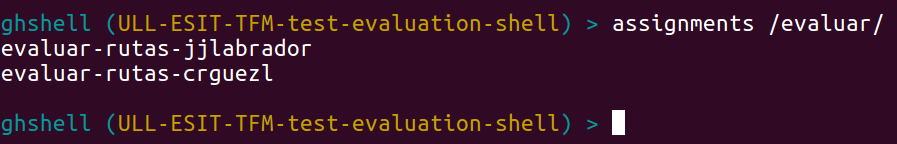
\includegraphics[width=0.8\textwidth]{images/assignments1-1}
		\caption{Assignments que coinciden con la expresión regular}
		\label{fig:assignment1-1}
		\end{center}
		\end{figure}
		
		
		En el caso de que además se pase alguno de los parámetros: 'clone', 'script \textless file\textgreater' o 'book'; se clonará, se ejecutará un script o se creará un libro respectivamente en los repositorios que coincidan con el string o la expresión regular. 
\bigskip		
		Además, en el caso del comando 'clone', se creará una carpeta con el nombre de la asignación que contendrá todas las asignaciones clonadas.
	
		\begin{figure}[H]
		\begin{center}
		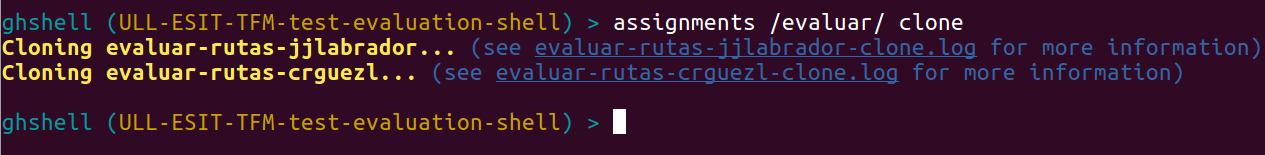
\includegraphics[width=1\textwidth]{images/ghshell6-1}
		\caption{Clonado de asignaciones que coinciden con la expresión regular}
		\label{fig:ghshell6-1}
		\end{center}
		\end{figure}
		
		\begin{figure}[H]
		\begin{center}
		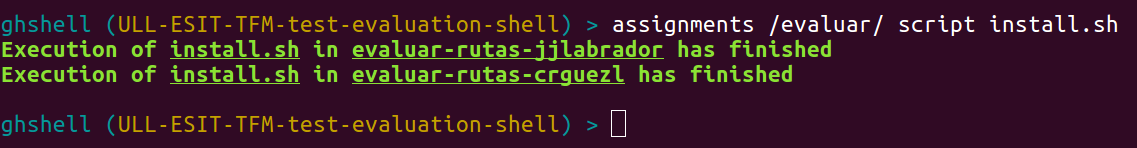
\includegraphics[width=1\textwidth]{images/assignments1-2}
		\caption{Ejecución de script en assignments que coinciden con la expresión regular}
		\label{fig:assignment1-2}
		\end{center}
		\end{figure}
		
		\begin{figure}[H]
		\begin{center}
		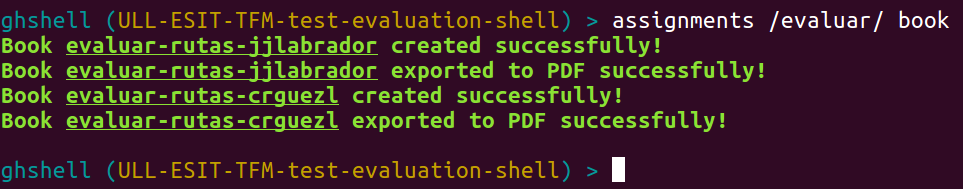
\includegraphics[width=1\textwidth]{images/assignments1-3}
		\caption{Creación del Gitbook en los assignments que coinciden con la expresión regular}
		\label{fig:assignment1-3}
		\end{center}
		\end{figure}
		
		\begin{figure}[H]
		\begin{center}
		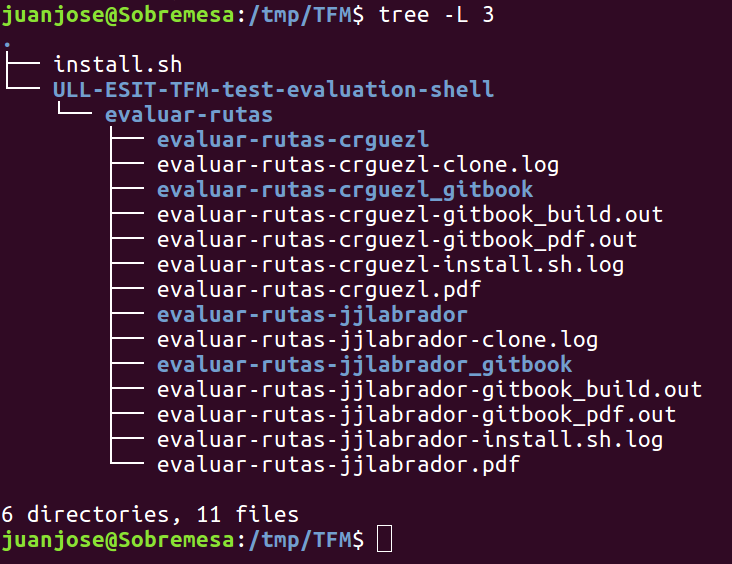
\includegraphics[width=0.7\textwidth]{images/assignments1-4}
		\caption{Directorios y ficheros generados}
		\label{fig:assignment1-4}
		\end{center}
		\end{figure}		
	
\end{itemize}

\subsection{Contexto de repositorio}
\label{subsec:b.2.3}

	Los comandos 'pwd' y 'exit' tienen el mismo comportamiento que en el contexto principal. 
	El comando 'back' tienen el mismo comportamiento que en el contexto de organizaciones.
	
\begin{itemize}

	\item Mostrar la ayuda. Comando 'help'.
		
		\begin{verbatim}
			ghshell > help
		\end{verbatim}
		
		En función del contexto donde nos encontremos, se mostrarán diferentes opciones en la ayuda.
				
		\begin{figure}[H]
		\begin{center}
		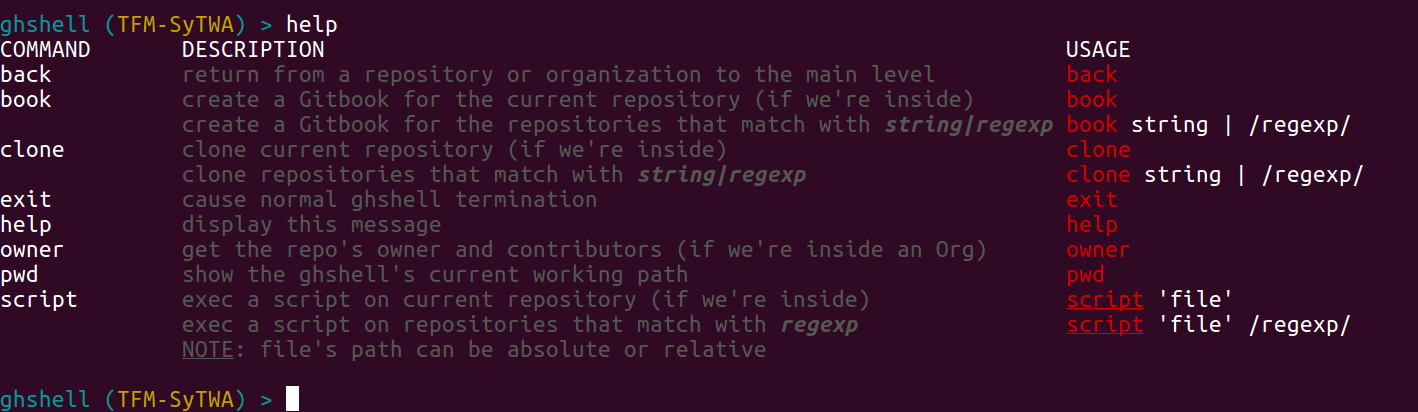
\includegraphics[width=1\textwidth]{images/help1-3}
		\caption{Ayuda en el contexto de un repositorio}
		\label{fig:help1-2}
		\end{center}
		\end{figure}

	%-------------------	
	\item Clonar repositorios. Comando 'clone'.
	
		\begin{verbatim}
			ghshell > clone
		\end{verbatim}
		
		Tiene el mismo funcionamiento que en el resto de contextos. Se ejecuta sin argumentos y clona el repositorio donde nos encontremos.
		
		\begin{figure}[H]
		\begin{center}
		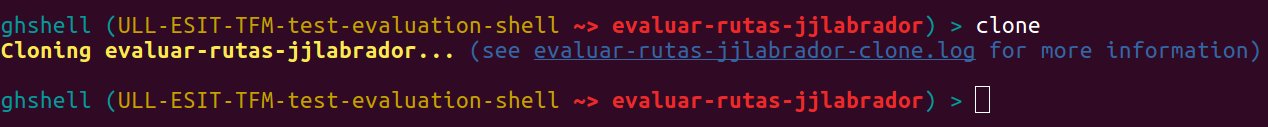
\includegraphics[width=1\textwidth]{images/clone1-4}
		\caption{Clonado de un repositorio dentro de una organización}
		\label{fig:clone1-4}
		\end{center}
		\end{figure}
		
	%-------------------		
	\item Ejecutar un script determinado. Comando 'script'
	
		\begin{verbatim}
			ghshell > script <file>
		\end{verbatim}
		
		Tiene el mismo funcionamiento que en el contexto de organizaciones. Se ejecuta sin argumentos y ejecuta el script indicado sobre el repositorio donde nos encontremos.
		
		\begin{figure}[H]
		\begin{center}
		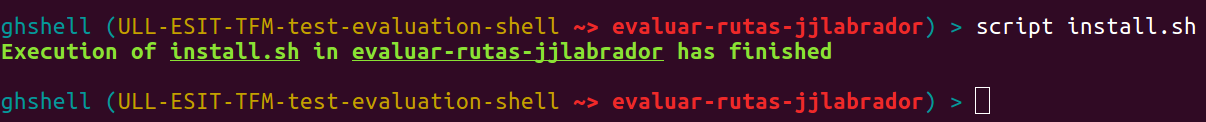
\includegraphics[width=1\textwidth]{images/script1-3}
		\caption{Ejecución de un script en un repositorio dentro de una organización}
		\label{fig:script1-3}
		\end{center}
		\end{figure}
		
	%-------------------
	\item Exportar resultados. Comando 'book'.
	
		\begin{verbatim}
			ghshell > book
		\end{verbatim}
		
		Tiene el mismo funcionamiento que en el contexto de organizaciones. Se ejecuta sin argumentos y crea un Gitbook con los resultados de todos los scripts ejecutados sobre el repositorio donde nos encontremos.
		
		\begin{figure}[H]
		\begin{center}
		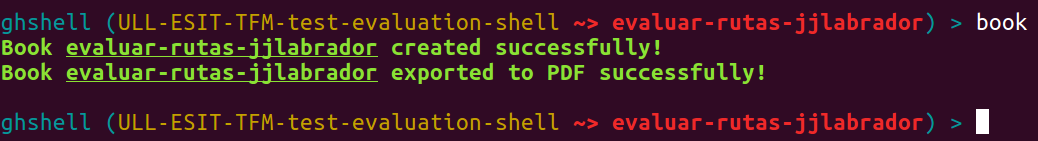
\includegraphics[width=1\textwidth]{images/book1-3}
		\caption{Creación del Gitbook en un repositorio dentro de una organización}
		\label{fig:book1-3}
		\end{center}
		\end{figure}
	
	%-------------------	
	\item Obtener el propietario del repositorio. Comando 'owner'.
	
		\begin{verbatim}
			ghshell > owner
		\end{verbatim}
		
		\begin{figure}[H]
		\begin{center}
		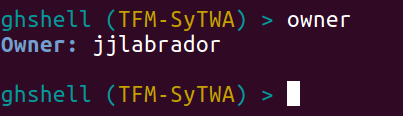
\includegraphics[width=0.5\textwidth]{images/owner1-1}
		\caption{Propietario del repositorio}
		\label{fig:owner1-1}
		\end{center}
		\end{figure}
		
		Además, si nos encontramos en un repositorio que pertenece a una organización, muestra también los contribuyentes.
		
		\begin{figure}[H]
		\begin{center}
		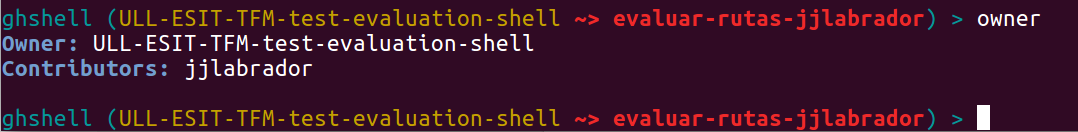
\includegraphics[width=1\textwidth]{images/owner1-2}
		\caption{Contribuyentes del repositorio}
		\label{fig:owner1-2}
		\end{center}
		\end{figure}
	
\end{itemize}



